% Document class `report-template` accepts either project-plan or final-report option in [].
\documentclass[project-plan]{report-template}

% Packages I use in my report.
\usepackage{graphicx}
\usepackage{amsmath}
\usepackage{blindtext}

% Directory where I saved my figures.
\graphicspath{{./figures/}}

% Metadata used for the title page - please modify.
\university{Imperial College London}
\department{Department of Earth Science and Engineering}
\course{MSc in Environmental Data Science and Machine Learning}
\title{Building a route optimisation system that takes elevation into consideration}
\author{Jinsong Dong}
\email{jinsong.dong22@imperial.ac.uk}
\githubusername{edsml-jd622}
\supervisors{Sesinam Dagadu\\
             Dr. Yves Plancherel}
\repository{https://github.com/ese-msc-2022/irp-jd622}

\begin{document}

\maketitlepage  % generate title page

% Abstract
\section* {Abstract}

% Introduction section
\section {Introduction}
\subsection {Literature Review}
The route optimisation problem in this project is a kind of Travel Salesman Problem(TSP) \cite{lawler1985travelling}, 
which means given a list of cities and distances between each pair of cities, what is the shortest possible
route that visits each city exactly once and returns to the origin city \cite{TSP_wiki}.\\

TSP is a classic NP-hard problem, means it can not be solved in polynomial time.
One example of a solution of a TSP is shown in Fig.~ \ref{fig:solution_of_TSP}.

\begin{figure}
    \begin{center}
        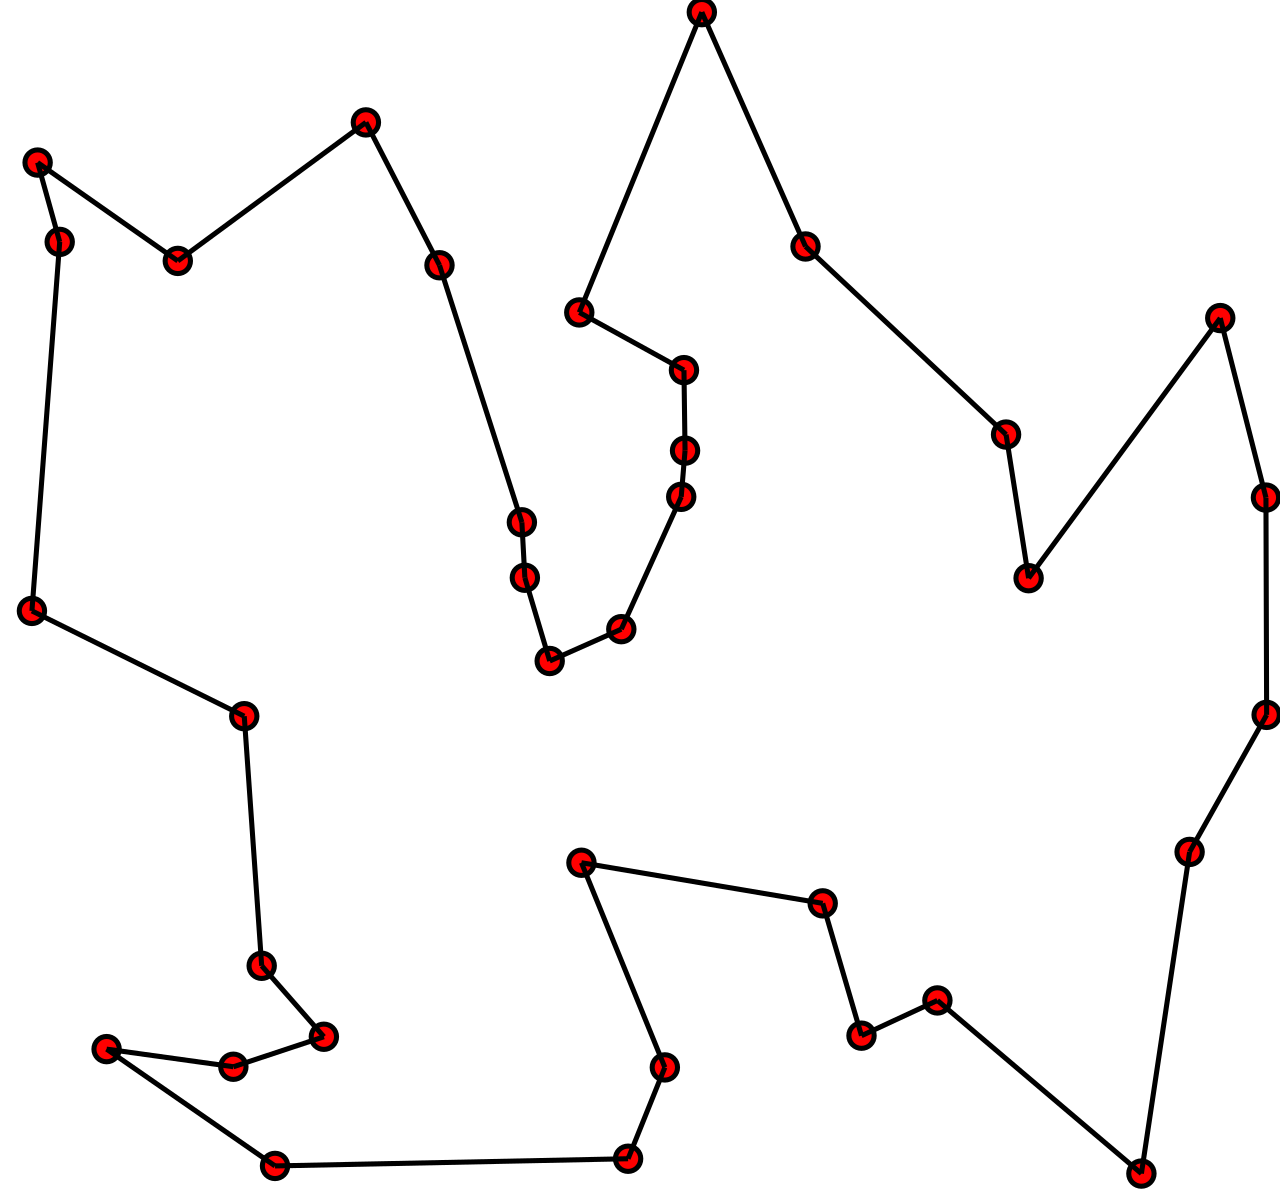
\includegraphics[width=0.2\textwidth]{solution_of_a_TSP.png}
    \end{center}
    \caption{\label{fig:solution_of_TSP} A solution example for TSP.}
\end{figure}

In this example, there are 35 locations in total, and the shortest way between these locations are drawn in the line.
There are $35!$ possible combination of the route totally, the 'brute-force solution' will take a very long time to get the results.\\

So algorithms to reduce the calculation time is essential. Many heuristic algorithms have been utilized in solving TSP\cite{TSP_review},
for example: ant algorithm, greedy method, simulated annealing, tabu search and genetic algorithm \cite{genetic_on_TSP}. \\

Genetic algorithm randomly samples values of the changing cells between lower and upper bounds to generate
a set of combination of possible route, and choose the best one.
Genetic algorithm can give a near to optimal solution in a relatively short time, but we cannot know how near it can be to the best route.\\

Ant Colony Optimization algorithm(ACO) is one of the metaheuristic methods for solving TSP, 
it works like observation of real ants, and upon finding food return to their colony while laying down pheromone trails\cite{ACO_on_TSP}. 
The ACO can also get a near-optimal solutions to the traveling salesman problem, it's able to find the global optimum in a finite time.
Some improved ACO algorithms have also been proposed like Parallel implementation of ant colony optimization \cite{para_ACO}. \\

Christofides algorithm\cite{VANBEVERN2020118} utilizes Minimum spanning tree(MST) to get the approximation solution of traveling salesman problem.
It is an approximation algorithm that guarantees its solutions will be within a factor of 3/2 of the optimal solution length.
Christofides algorithm has the limitation that it can only be applied on the instances where the distances form a metric space(they are symmetric and obey the triangle inequality) \cite{christofides_inbook}.
The project satisfies the condition as it is based on the distances between different locations.\\

Simulated annealing(SA) algorithm is a kind of greedy algorithms. It uses randomness as part of its search for the best solution, so it is a stochastic global search algorithm.
Simulated annealing algorithm is good at jumping out of the local minimum\cite{improved_SA}, 
to achieve this, SA accepts worse candidates with a probability dependent on the control variable, the probability is calculated based on the equation below:\\

\begin{equation}
    p =
    \begin{cases}
    1, & \text{if } f(y) \geq f(x) \\
    e^{-(f(y)-f(x)) / T}, & \text{otherwise}\\
    \end{cases}
\end{equation}

In the equation, \\
$p$ is the probability of accepting the new solution candidate $y$,\\
$f$ is the function that measures the performance of the solution candidate (In this project, length of the routes),\\
$T$ is the control parameter, which is a hyperparameter.\\

The algorithms mentioned above all have their own pros and cons. In this project, Christofides algorithm and Christofides algorithm will be implemented.



\subsection {Problem Description}
Snoocode Corporation has designed a route optimization system that works offline on a smartphone and provides 
results 42000 times faster than the conventional method. However, this method only consider a 2D map.
The next step for Snoocode is developing and incorporate an algorithm that considers land elevation. 
In this method, I need to optimize the route in a 3D map, as elevation is a very important factor for 
electric bikes and bicycles. \\

To be more specific about the function of the route optimisation system, suppose we have 20 locations to
give delivery to, we need to find the shortest way to go so that we can deliver to every location. 
But in this case, a very important thing is to consider altitude, 
Because there will be two points that are close in the projection direction toward the ground, 
but have a large difference in elevation. In this case, we cannot simply go in the way between the two locations.
Instead, we might take a long detour to make the ascent of way between the two locations less steep.\\

In this project, I simplify the problem as a single 3D TSP, try to implement two algorithms to solve the problem.
The algorithm can output the possible shortest route given a list of coordinates of some locations
(x, y, z) with altitude in consideration.

\subsection {Objectives}
The project has four objectives below:
\begin{itemize}
    \item Implementing the 3D Christofides algorithm on a TSP with 20 points list of virtual coordinates.
    \item Implementing the 3D Simulated Annealing algorithm on a TSP with 20 points list of virtual coordinates.
    \item Evaluating the two algorithms above and the other two algorithms implemented by another student.
    \item Expanding the two algorithms above on the locations in a real-world case (more complicated coordinates).
\end{itemize}

\section {Progress to Date}
\begin{itemize}
    \item 29/May - 5/June: The draft of the project plan.
    \item 6/June - 14/June: Literature review and modify the project plan.
    \item 15/June - 29/June: Implementing the 2D version of Christofides and Simulated Annealing on a given list of locations.
    \item 29/June - 13/July: Implementing the 3D version of Christofides and Simulated Annealing on a given list of locations.
    \item 13/July - 31/July: Expanding these 3D algorithms on the locations in a more complicated coordinates.
    \item 31/July - 15/August: Write tests.
    \item 15/August - 1/September: Prepare all files needed to be submitted.
\end{itemize}

\section {Future Plan}
If there is time after implementing two 3D algorithms on the route optimisation system with altitude in
consideration, the next step is to write a machine learning model or deep learning model
to improve the result of the system. \\

Reinforcement model is a consideration of priority, as it may be hard to get the training dataset.
To train the reinforcement model in this project, I need to build a reinforcement learning agent that can
interact with the environment and learns to choose the optimal order of city visits. 
The agents can select the next city it visits based on the current state(the current city it's in), 
and finally evaluates and optimizes the selection based on the reward signals(the path length and elevation).


% References
\bibliographystyle{plain}
\bibliography{references}  % BibTeX references are saved in references.bib

\end{document}          
